\documentclass[12pt,letterpaper]{article}
\usepackage{graphicx,textcomp}
\usepackage{natbib}
\usepackage{setspace}
\usepackage{fullpage}
\usepackage{color}
\usepackage[reqno]{amsmath}
\usepackage{amsthm}
\usepackage{fancyvrb}
\usepackage{amssymb,enumerate}
\usepackage[all]{xy}
\usepackage{endnotes}
\usepackage{lscape}
\newtheorem{com}{Comment}
\usepackage{float}
\usepackage{hyperref}
\newtheorem{lem} {Lemma}
\newtheorem{prop}{Proposition}
\newtheorem{thm}{Theorem}
\newtheorem{defn}{Definition}
\newtheorem{cor}{Corollary}
\newtheorem{obs}{Observation}
\usepackage[compact]{titlesec}
\usepackage{dcolumn}
\usepackage{tikz}
\usetikzlibrary{arrows}
\usepackage{multirow}
\usepackage{xcolor}
\newcolumntype{.}{D{.}{.}{-1}}
\newcolumntype{d}[1]{D{.}{.}{#1}}
\definecolor{light-gray}{gray}{0.65}
\usepackage{url}
\usepackage{listings}
\usepackage{color}
 
\definecolor{codegreen}{rgb}{0,0.6,0}
\definecolor{codegray}{rgb}{0.5,0.5,0.5}
\definecolor{codepurple}{rgb}{0.58,0,0.82}
\definecolor{backcolour}{rgb}{0.95,0.95,0.92}
 
\lstdefinestyle{mystyle}{
    backgroundcolor=\color{backcolour},   
    commentstyle=\color{codegreen},
    keywordstyle=\color{magenta},
    numberstyle=\tiny\color{codegray},
    stringstyle=\color{codepurple},
    basicstyle=\footnotesize,
    breakatwhitespace=false,         
    breaklines=true,                 
    captionpos=b,                    
    keepspaces=true,                 
    numbers=left,                    
    numbersep=5pt,                  
    showspaces=false,                
    showstringspaces=false,
    showtabs=false,                  
    tabsize=2
}
 \lstset{style=mystyle}
\newcommand{\Sref}[1]{Section~\ref{#1}}
\newtheorem{hyp}{Hypothesis}

\title{Text as Data: Homework 5}
\date{August 23, 2017}
\author{Jeff Ziegler}

\begin{document}
\maketitle


\section{Using the {\tt Structural Topic Model} in {\tt R}}
Using the preprocessed data based on the NYT Json file and the subsequent document term matrix for analysis in {\tt stm}.

\begin{itemize}
\item[a)] Download the {\tt stm} package for {\tt R} from {\tt CRAN}
\item[b)] Convert the document-term matrix to the appropriate format.  To do this, create a list in {\tt R} where each component of the list corresponds to an individual document.  Store in each component of the list a two rom matrix.  The number of columns corresponds to the number of non-zero entries for the document in the document-term matrix.  The first row will describe the words used in the document (the columns with the non-zero entry).  The second row will correspond to a count of each of the words in the document (they should all be non-zero)
\item[c)] Following the help file in {\tt STM} fit a model with 8 topics that conditions on the {\tt desk} of origin for topic prevalence
\item[d)] Use {\tt labelTopics} to label each of the topics
\item[e)] Compare the 8 topic proportions for each document to the 8 topic proportions without conditioning on {\tt desk} (in vanilla LDA).  How do the results differ?
\end{itemize}

\lstinputlisting[language=R, firstline=1, lastline=100]{WUSTL_HW5_JZ.r}  

\begin{figure}[H]
  \caption{\footnotesize{Example documents highly associated with topics.}}
  \centering
   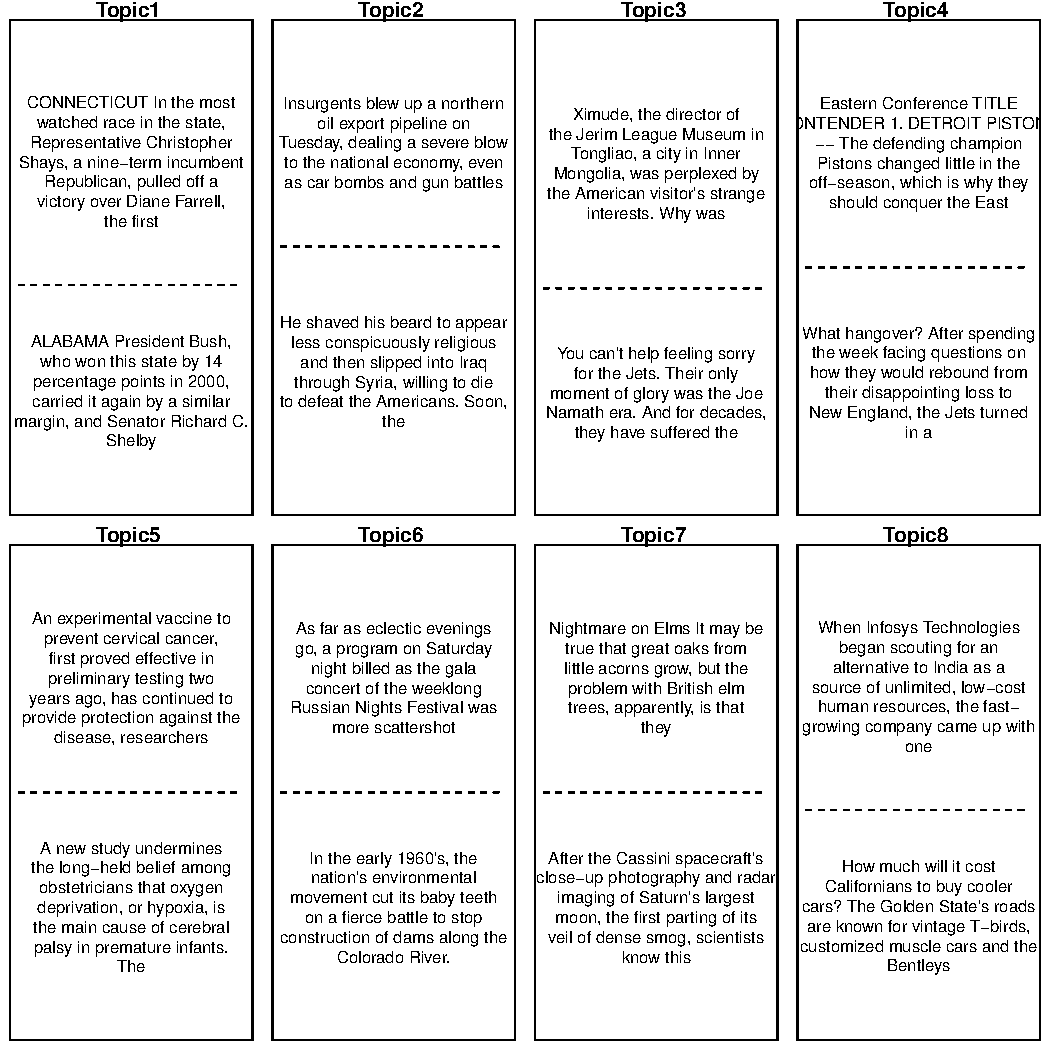
\includegraphics[width=.75\linewidth]{HW5topicReview.pdf}\\
\end{figure}

\begin{figure}[H]
  \caption{\footnotesize{Expected distribution of topic proportions across the documents, vanilla LDA vs. conditioning on {\tt desk} .}}
  \centering
   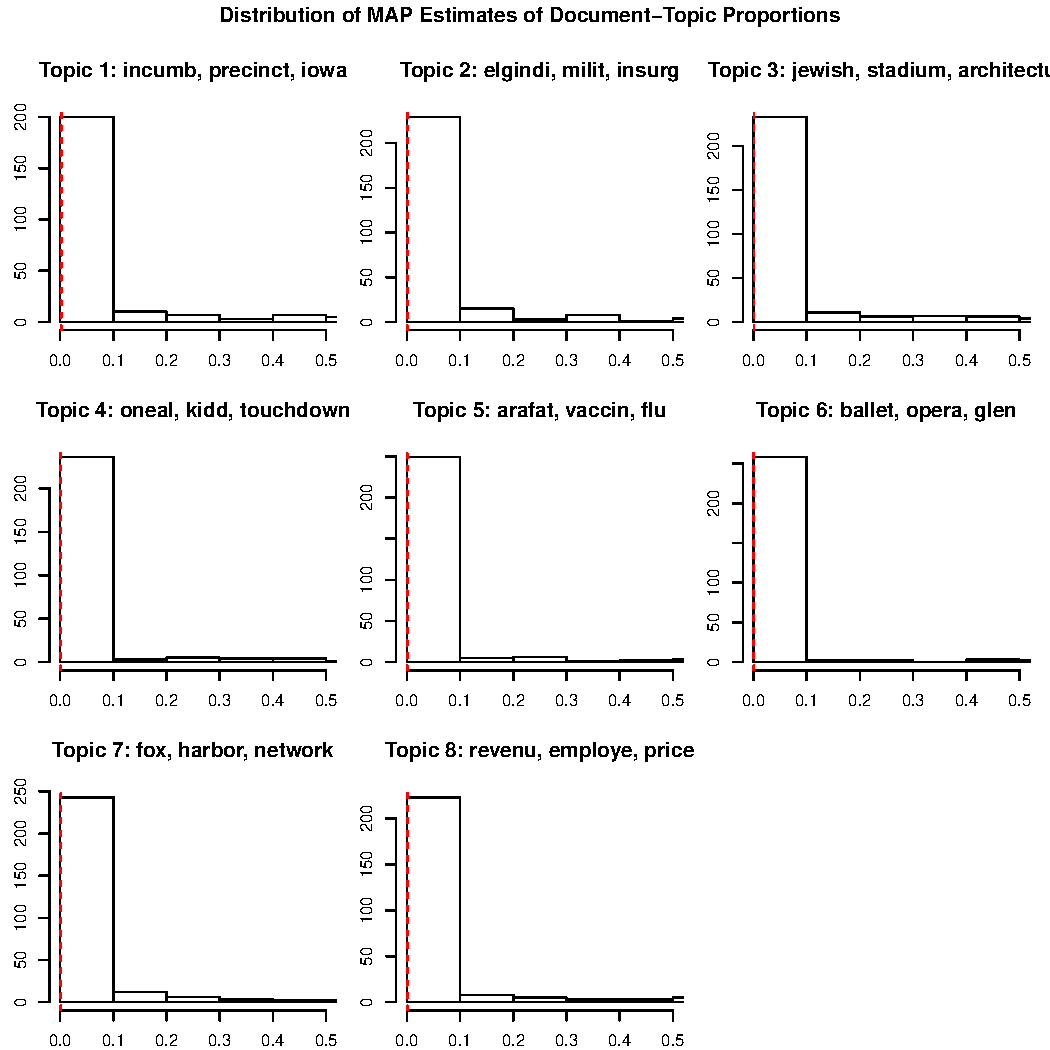
\includegraphics[width=.49\linewidth]{HW5topicProportionsSTM.pdf}
      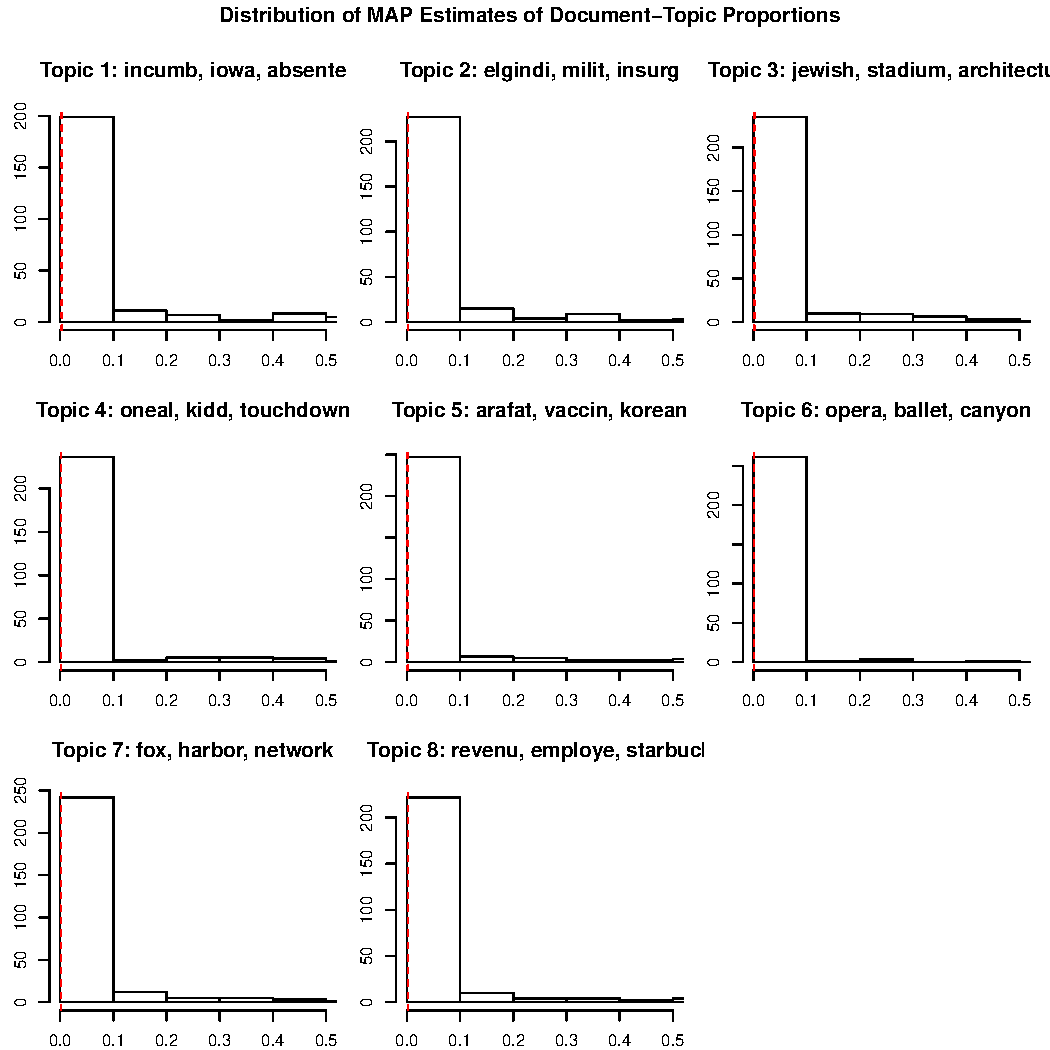
\includegraphics[width=.49\linewidth]{HW5topicProportionsLDA.pdf}\\
\end{figure}

\section{Machiavelli's Prince}


In this part of the assignment we will analyze Machiavelli's \emph{The Prince}.  Download {\tt Mach.tar} from the course website and expand the compressed folder.  (This is relevant {\tt http://xkcd.com/1168/}).  \\

Each file represents a subset of the manuscript.  We will analyze its contents using principal components, multidimensional scaling, and clustering methods.



\subsection*{Create a Document-Term Matrix}

Using the sections from the Machiavelli text, create a document term matrix.
\begin{itemize}
\item[-] Discard punctuation, capitalization
\item[-] Apply the porter stemmer to the documents
\item[-] Identify the 500 most common unigrams
\item[-] Create a $N \times 500$ document term matrix $\boldsymbol{X}$, where the columns count the unigrams and the rows are the documents
\end{itemize}


We will work with a normalized version of the term document matrix.  That is we will divide each row by the total number of words in the top 500 unigrams used:
\begin{eqnarray}
\boldsymbol{x}_{i}^{*} & = & \frac{\boldsymbol{x}_{i}}{\sum_{j=1}^{500} x_{ij}} \nonumber\\
\boldsymbol{X}^{*} & = & \begin{pmatrix} \boldsymbol{x}_{1}^{*} \\
\boldsymbol{x}_{2}^{*} \\
\vdots \\
\boldsymbol{x}_{N}^{*} \\
  \end{pmatrix}  \nonumber
\end{eqnarray}




\subsection*{Low Dimensional Embeddings with Principal Components}

\begin{itemize}
\item[1)]  Wise Will (WW), your friend with a weird name, notices you looking at the slides about principal component analysis (PCA).   WW casually remarks that the variance of the eigenvalues of the variance-covariance matrix is a useful heuristic for knowing if PCA can be fruitfully applied to some document-term matrix.  WW, completely unsolicited, explains that as the variance of the eigenvalues goes up, the more useful PCA will be.  He then laughs and leaves your office.  WW is kind of a jerk.   \\

Let's formalize WW's suggestion. Suppose document-term matrix $\boldsymbol{X}$ has variance-covariance matrix $\boldsymbol{\Sigma} = \frac{\boldsymbol{X}^{'}\boldsymbol{X}}{N}$.  And suppose that $\boldsymbol{\Sigma}$ has eigenvalues $\lambda_{1}>\lambda_{2}>\hdots > \lambda_{d}>0$. Then we calculate the variance of the eigenvalues as
\begin{eqnarray}
\sigma^{2} & = & \frac{1}{d} \sum_{j=1}^{d}(\lambda_{j} - \bar{\lambda})^{2} \nonumber
\end{eqnarray}

where $\bar{\lambda}$ is $\frac{1}{d} \sum_{i=1}^{d} \lambda_{i}$. WW is saying that as $\sigma^{2}$ gets bigger, a low-dimensional embedding via PCA will provide a better summary of our data.   \\

Does WW have a good point?  Why or why not? (Hint: what do the eigenvalues represent?)
\item[2)] Apply the function {\tt prcomp} to $\boldsymbol{X}^{*}$. Be sure to set use a scaled version of the data, by setting {\tt scale = T}, which will ensure that each column has unit variance.
\begin{itemize}
\item[a)] Create a plot of variance explained by each additional principal component. What does this plot suggest about the number of components to include?
\item[b)] Plot the two-dimensional embedding of the text documents.  Label the texts with their number.  (Each file is {\tt Mach\_XX.txt}, where {\tt XX} is the chunk number)
\item[c)] Label the two largest principal components.  What does this embedding suggest about the primary variation this representation of the Prince?  (Hint: if your {\tt embed} is your object with principal components, examine {\tt embed\$rotation})
\end{itemize}


\item[3)]An alternative method---discussed at the end of the seventh lecture---is multidimensional scaling (MDS).  Classic MDS attempts to preserve distances between objects in a low dimensional scaling.

\begin{itemize}
\item[a)] Calculate the Euclidean distance between each document using $\boldsymbol{X}^{*}$.  Call this matrix $\boldsymbol{D}(\boldsymbol{X}^{*})$  (Hint: use {\tt R}'s built in function {\tt dist})
\item[b)] Apply the classic MDS to $\boldsymbol{D}(\boldsymbol{X}^{*})$ using the {\tt R} function {\tt cmdscale}.  That is, execute the code\\
{\tt mds\_scale<- cmdscale(DISTANCE\_MATRIX, k = 2)}
\item[c)] Apply PCA to $\boldsymbol{X}^{*}$, but this time do not use {\tt prcomp}'s scaling option.  That is, use {\tt prcomp} with {\tt scale = F}.
\item[d)] Compare the first dimension of the output from classic MDS to the first dimension of the embedding from principal components. What is the correlation between the embeddings?
\item[d)] Now use {\tt dist} to create a distance matrix using the {\tt manhattan} metric, apply Classic multidimensional scaling to the distance matrix based on manhattan distance, and compare the first dimension of this embedding to the first dimension from PCA.  What is the correlation?
\item[e)] What do you conclude about the relationship between PCA and MDS?
\end{itemize}

\end{itemize}




\end{document}
